    \documentclass{article}
    \usepackage{fancyhdr, amsmath, amsthm, amssymb, mathtools, lastpage, hyperref, enumerate, graphicx, setspace, upgreek}
    \usepackage[margin=1in, top=0.8in,bottom=0.8in]{geometry}
    \usepackage{subcaption}
    \newcommand{\scinot}[2]{#1\times10^{#2}}
    \newcommand{\bra}[1]{\left<#1\right|}
    \newcommand{\ket}[1]{\left|#1\right>}
    \newcommand{\dotp}[2]{\left<#1\,\middle|\,#2\right>}
    \newcommand{\rd}[2]{\frac{\mathrm{d}#1}{\mathrm{d}#2}}
    \newcommand{\pd}[2]{\frac{\partial#1}{\partial#2}}
    \newcommand{\rtd}[2]{\frac{\mathrm{d}^2#1}{\mathrm{d}#2^2}}
    \newcommand{\ptd}[2]{\frac{\partial^2 #1}{\partial#2^2}}
    \newcommand{\norm}[1]{\left|\left|#1\right|\right|}
    \newcommand{\abs}[1]{\left|#1\right|}
    \newcommand{\pvec}[1]{\vec{#1}^{\,\prime}}
    \newcommand{\tensor}[1]{\overleftrightarrow{#1}}
    \let\Re\undefined
    \let\Im\undefined
    \newcommand{\ang}[0]{\text{\AA}}
    \newcommand{\mum}[0]{\upmu \mathrm{m}}
    \DeclareMathOperator{\Re}{Re}
    \DeclareMathOperator{\Tr}{Tr}
    \DeclareMathOperator{\Im}{Im}
    \DeclareMathOperator{\E}{E}
    \DeclareMathOperator{\Var}{Var}
    \newcommand{\expvalue}[1]{\left<#1\right>}
    \usepackage[labelfont=bf, font=scriptsize]{caption}\usepackage{tikz}
    \usepackage[font=scriptsize]{subcaption}
    \everymath{\displaystyle}

\begin{document}
\title{Ph20.2 - Introduction to Numerical Techniques:\\ Numerical Integration}
\author{Cassidy Yang}
\maketitle
\pagestyle{fancy}
\rhead{Cassidy Yang}
\cfoot{Page \thepage \hspace{1pt} of \pageref{LastPage}}

\section{The Assignment}

The corresponding Python code is attached in a separate document.

\subsection{Part 1}

\begin{enumerate}
	\item The equation for the mass on a spring is
	
	\begin{equation}
		F = ma = -kx.
	\end{equation}
	Additionally, we can apply $v = \frac{dx}{dt}$ and $a = \frac{dv}{dt} = \frac{-kx}{m}$ and use the explicit Euler method to approximate $x$ and $v$ as a function of time. Figure \ref{fig:x_exp} and Figure \ref{fig:v_exp} plots the approximated positions and velocities respectively ($h = 0.01$, $x_0 = 0$, $v_0 = 1$, $\frac{k}{m} = 1$). Note that after a few oscillations, the amplitudes increase noticeably, indicating a divergence from the exact solution and an increasing error.
	
	\begin{figure}[ht!]
		\centering
		\begin{subfigure}{0.4\textwidth}
		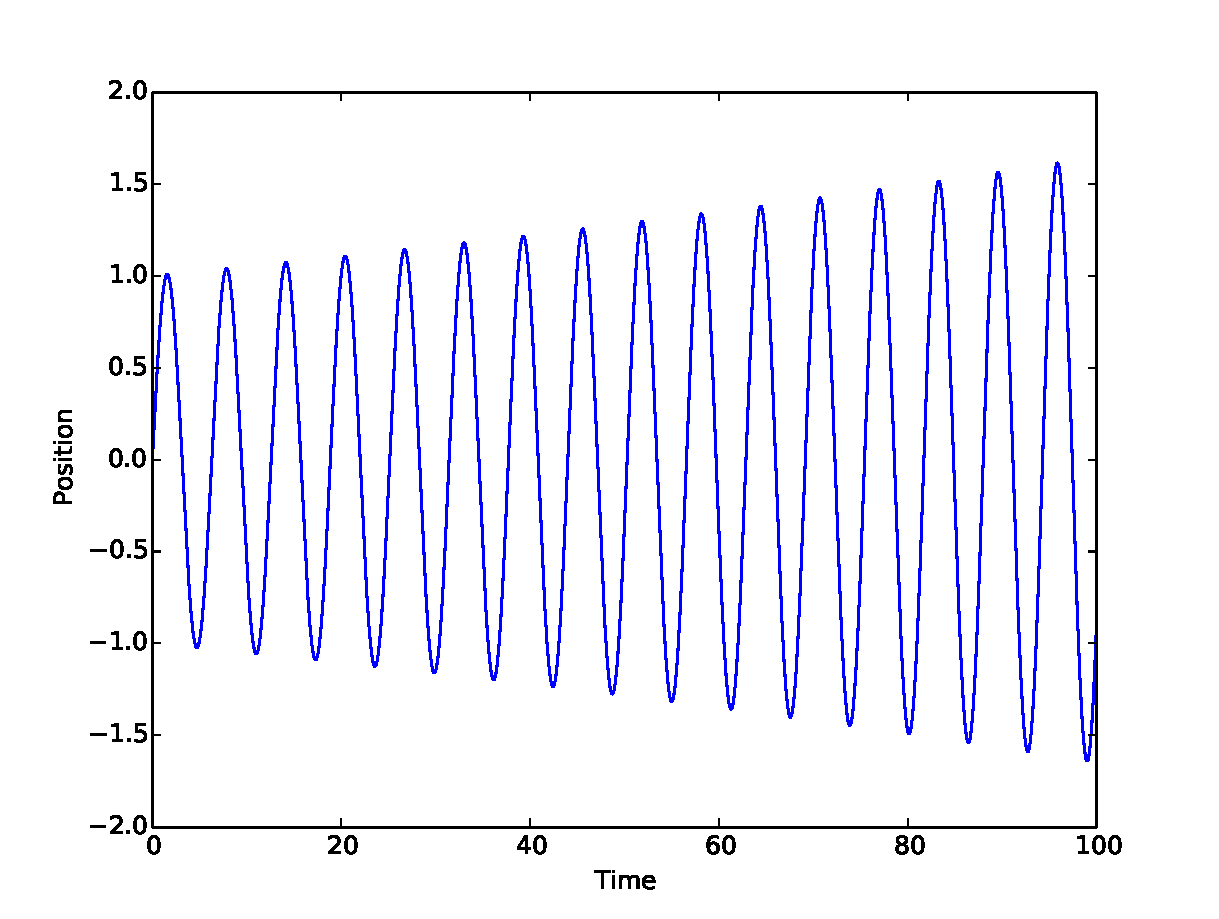
\includegraphics[width=2.2in]{position.pdf}
		\caption{}
		\label{fig:x_exp}
		\end{subfigure}
		~
		\begin{subfigure}{0.4\textwidth}
		\centering
		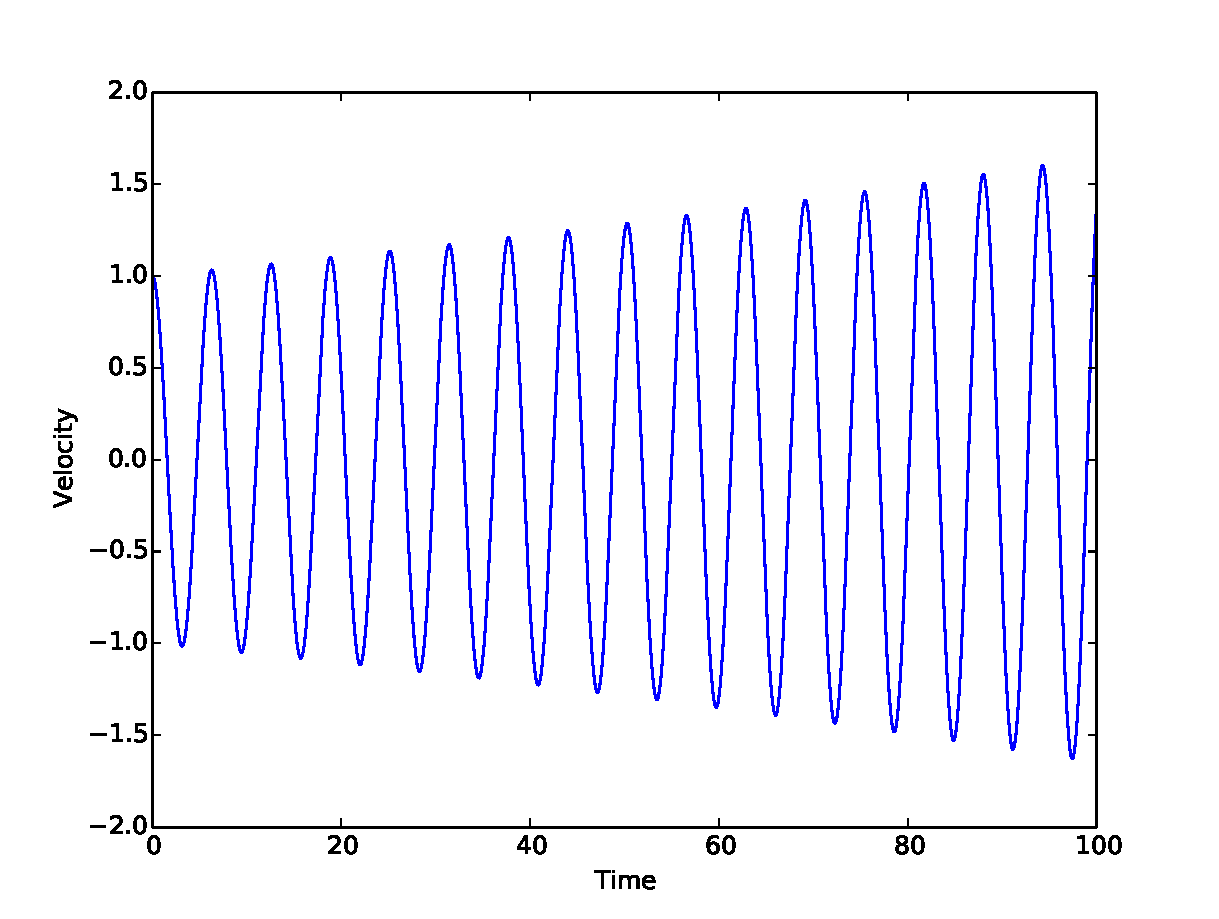
\includegraphics[width=2.2in]{v.pdf}
		\caption{}
		\label{fig:v_exp}
		\end{subfigure}
		\caption{Approximate Position and Velocity vs Time (Explicit Euler's Method)}
	\end{figure}
	
	\item We use the same parameters as above. The exact analytical solution for the initial conditions we use are $x_{anal}(t_i) = \sin t_i$ and $v_{anal}(t_i) = \cos t_i$. The growth of the global errors for our approximations of position (blue) and velocity (green) are shown in Figure \ref{fig:error}.
	
	\begin{figure}[ht!]
		\centering
		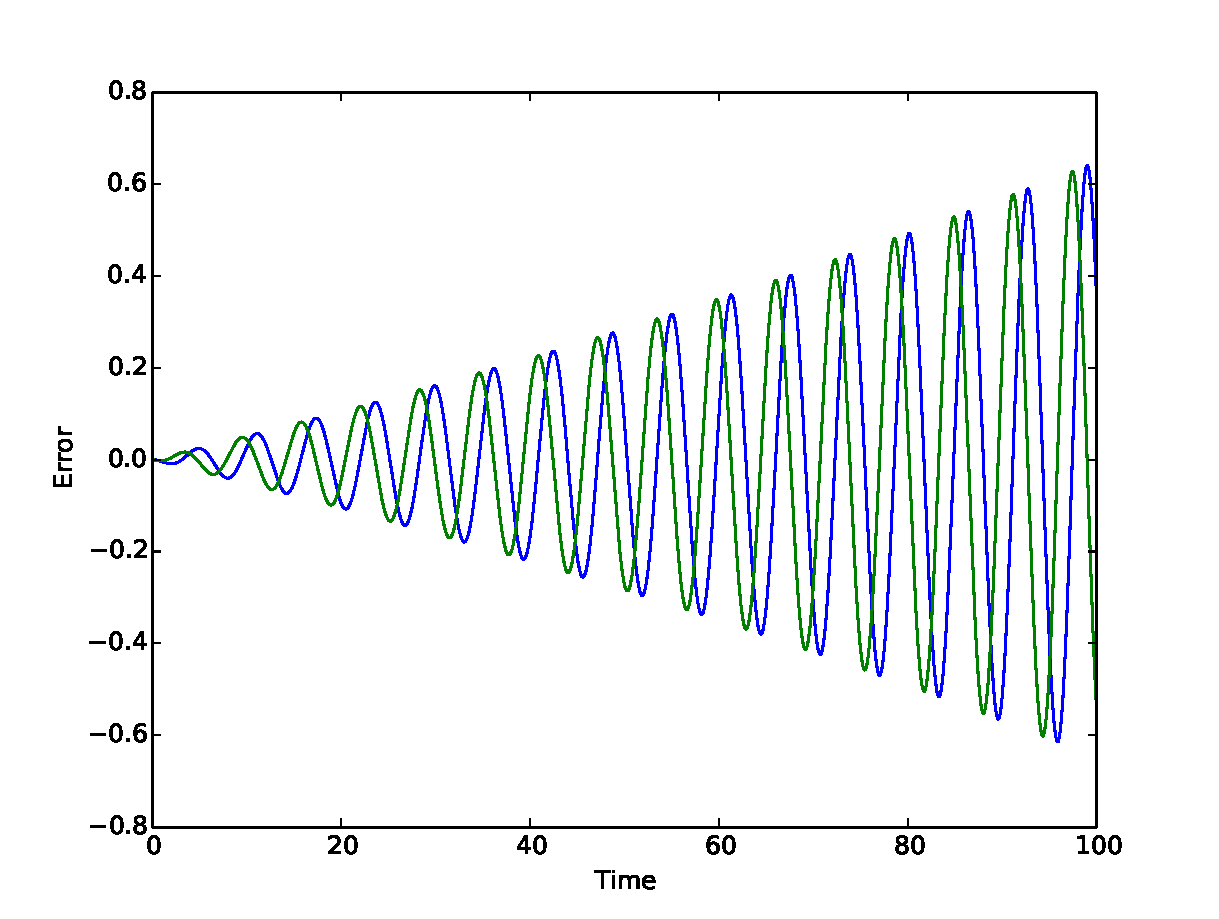
\includegraphics[width=3in]{errors.pdf}
		\caption{Errors in Position and Velocity vs. Time}
		\label{fig:error}
	\end{figure}
	
	\item The errors also vary with step size. We began with step size $h = 0.1, \frac{0.4}{2}, \frac{0.4}{2^2},$ etc. and extracted maximal absolute error in position from $t = 0$ to $t = 100$. Figure \ref{fig:stepsize} plots the maximal error as a function of step size. For small step sizes, the maximum error in position seems to decrease approximately linearly.
	
	\begin{figure}[ht!]
		\centering
		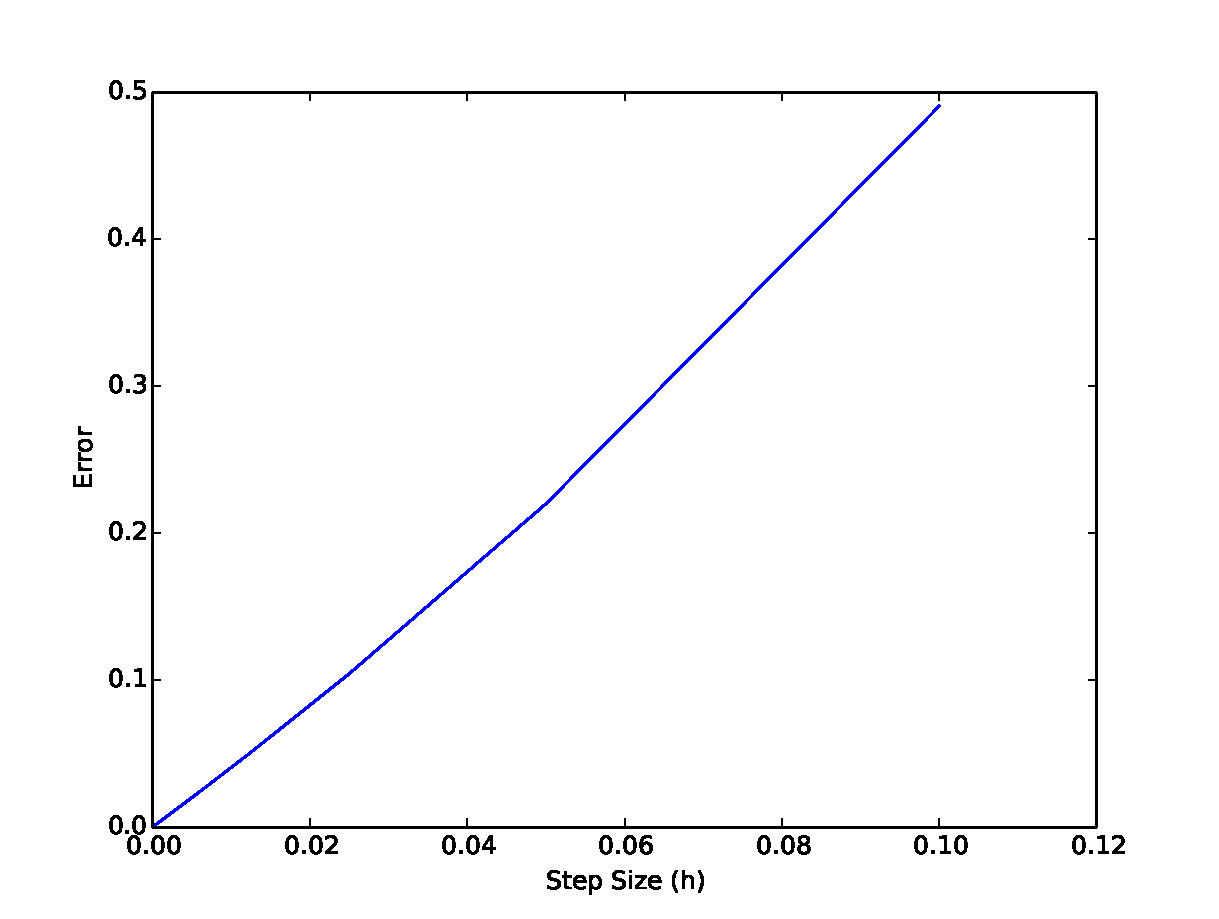
\includegraphics[width=3in]{stepsize.pdf}
		\caption{Maximum $x$ Error vs. Step Size}
		\label{fig:stepsize}
	\end{figure}
	
	\item The normalized total energy of the system can be calculated using $E = x^2 + v^2$ and observe the evolution of energy in time (Fig \ref{fig:energye}). The overall energy of the analytically solved system will always be $E = 1$, and we can also plot the error of $E$ (green) as a function of time and compare it to the absolute errors in position (blue) in Fig \ref{fig:energyerror_e}. Note that the error in energy increases much faster than that of position. 
	
	\begin{figure}[ht!]
		\centering
		\begin{subfigure}{0.4\linewidth}
		\centering
		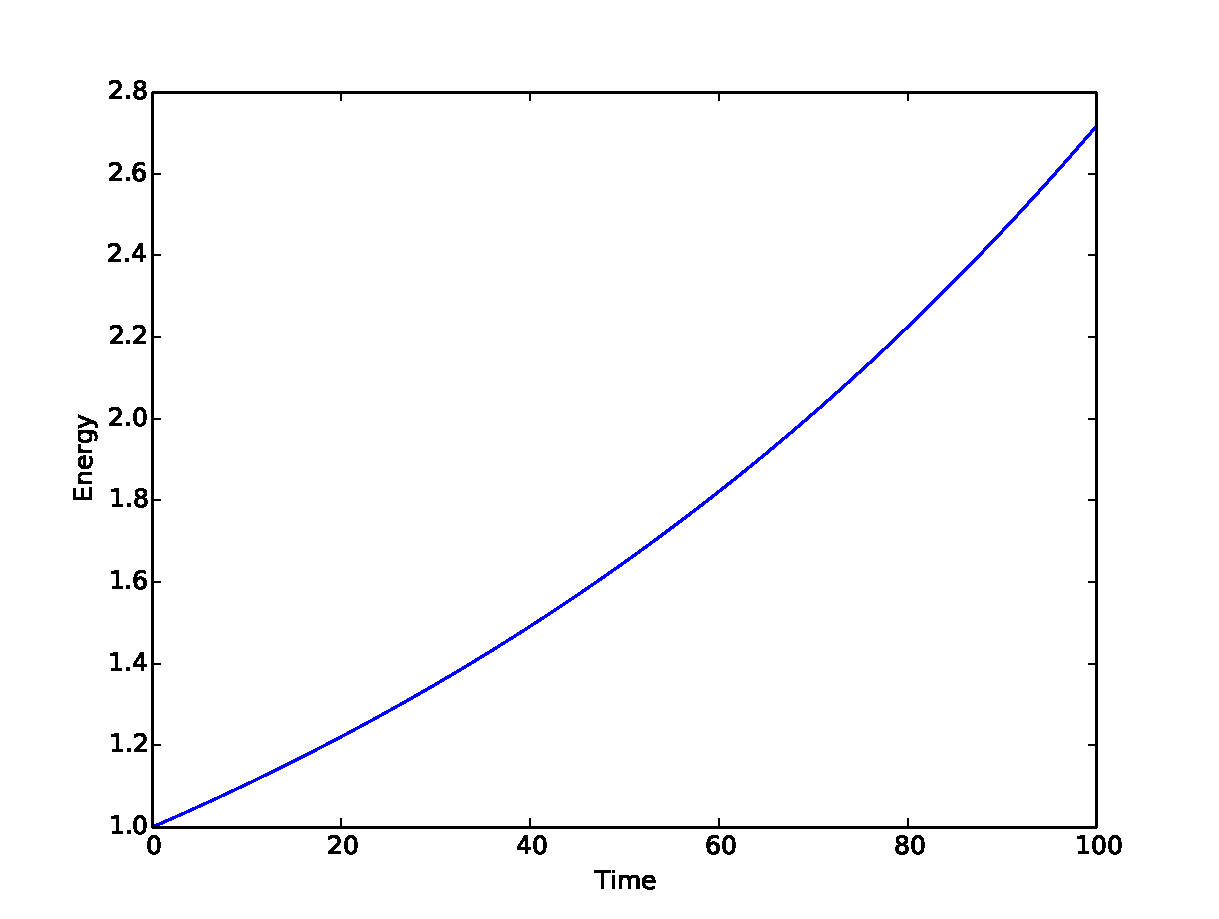
\includegraphics[width=2in]{energy_e.pdf}
		\caption{Energy vs Time}
		\label{fig:energye}
		\end{subfigure}
		~
		\begin{subfigure}{0.4\linewidth}
		\centering
		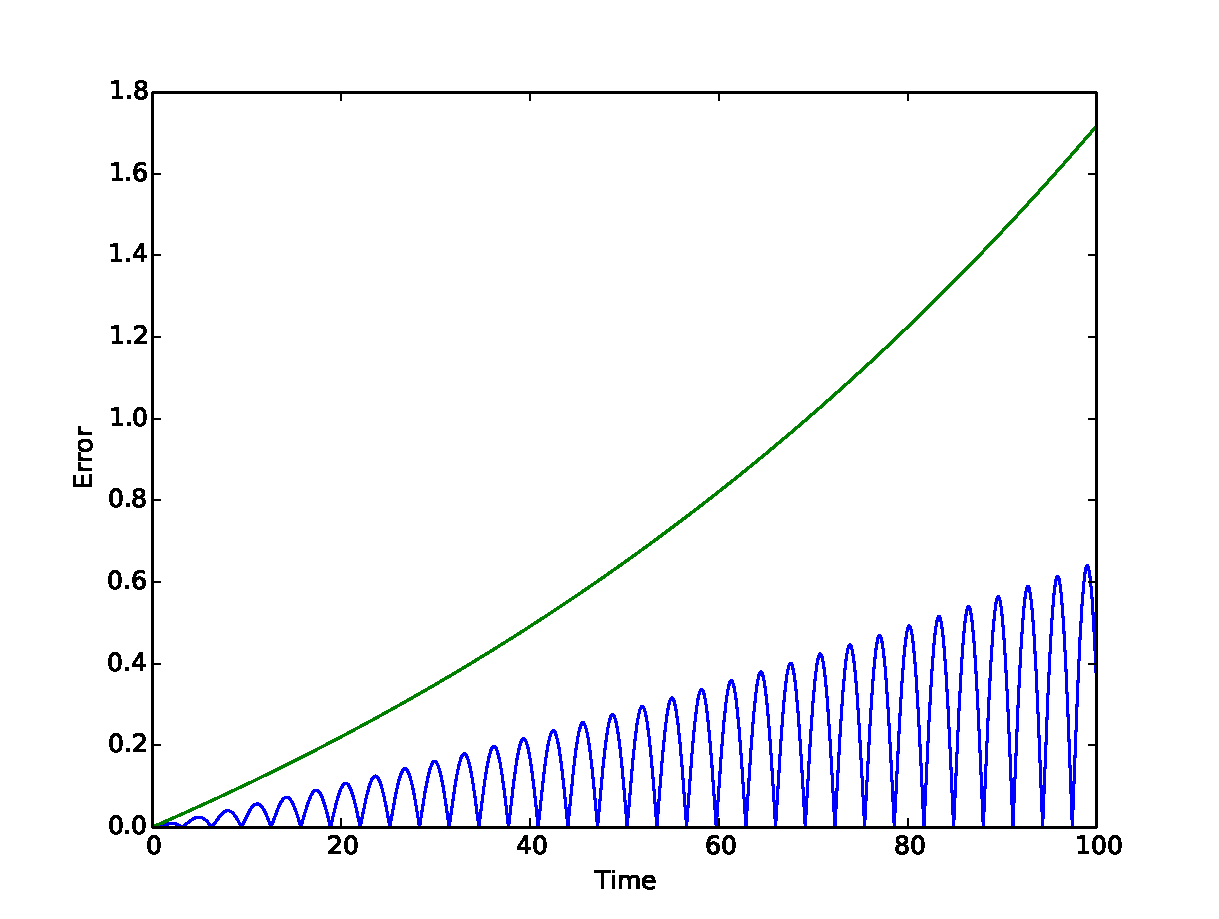
\includegraphics[width=2in]{energyerror_e.pdf}
		\caption{Errors vs Time}
		\label{fig:energyerror_e}
		\end{subfigure}
		\caption{Explicit Energy and Errors vs Time}
	\end{figure}
	
	\item Consider the implicit Euler's method, which has the following system
	
	\begin{equation}
		x_{i+1} = x_i + hv_{i+1}, \hspace{5pt} v_{i+1} = v_i - hx_{i+1}.
	\end{equation}
	
	We substitute the second equation into the first to solve the system to get the following explicit expressions for $x$ and $v$.
	
	\begin{align}
		x_{i + 1} &= \frac{x_i + hv_i}{h^2 + 1} \\
		v_{i+1} &= v_i - hx_{i+1} = v_i - h\left( \frac{x_i+hv_i}{h^2+1} \right)
	\end{align}
	
	The position and velocities are shown in Figure \ref{fig:implicit}. Note that the amplitudes decrease over time, indicating that the approximated energies will also decrease over time. 
	
	\begin{figure}[ht!]
		\centering
		\begin{subfigure}{0.4\linewidth}
		\centering
		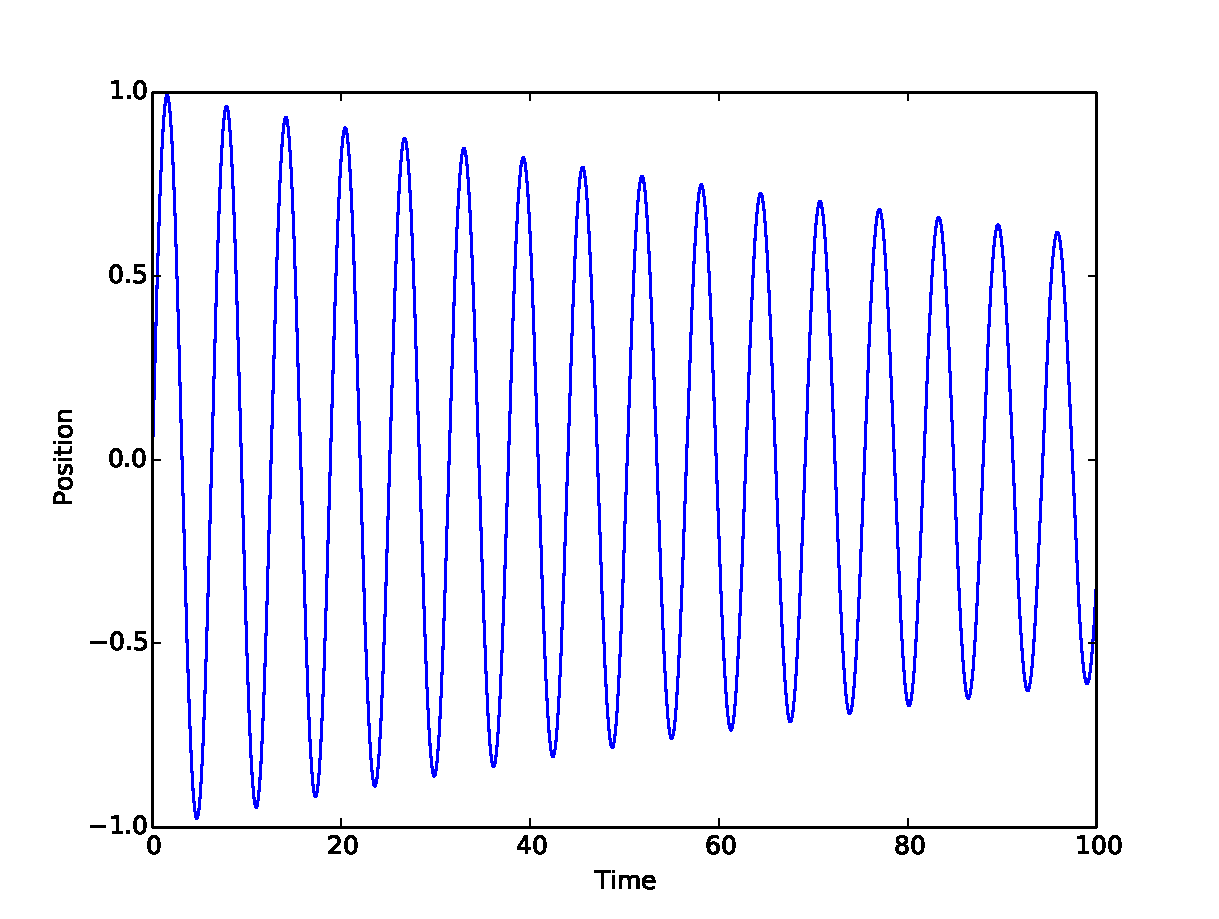
\includegraphics[width=2in]{p_i.pdf}
		\caption{}
		\end{subfigure}
		~
		\begin{subfigure}{0.4\linewidth}
		\centering
		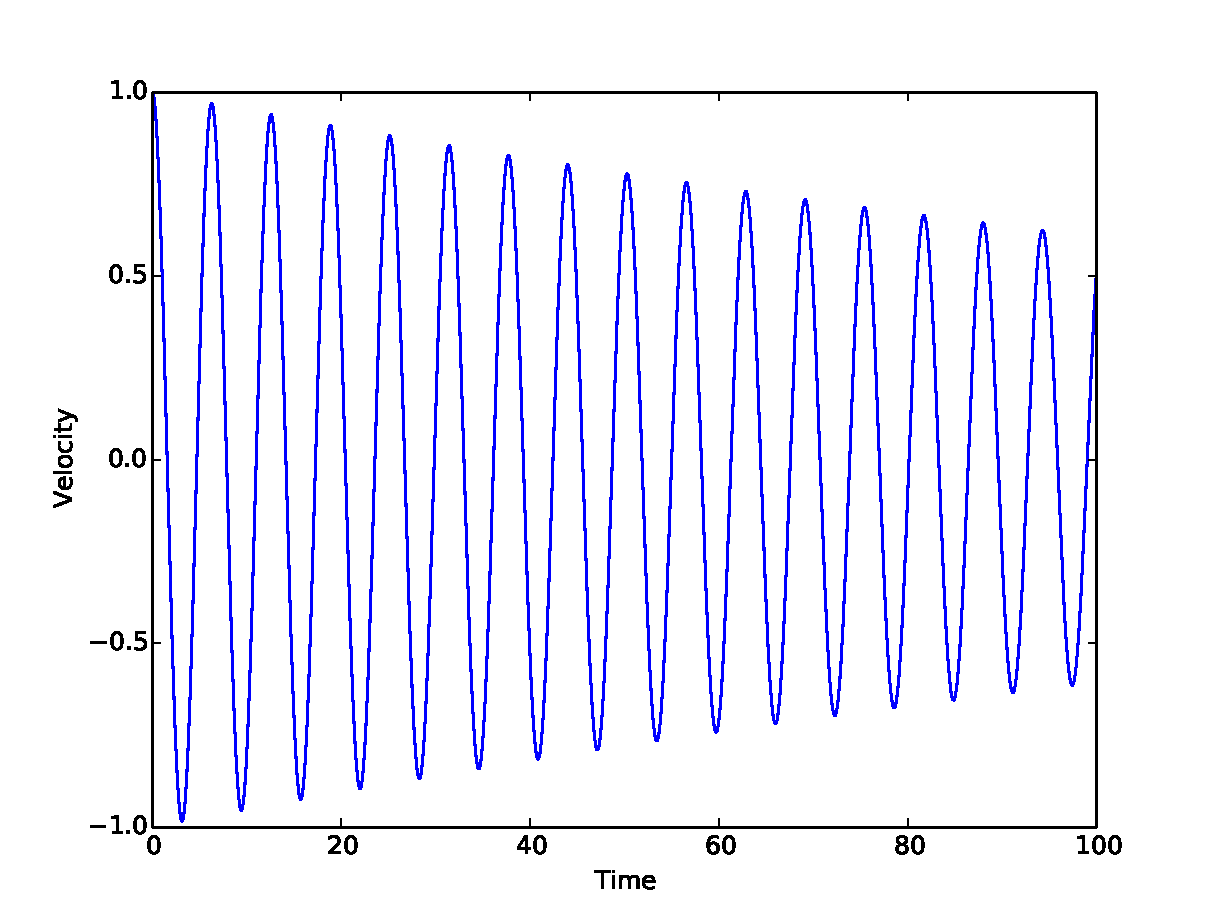
\includegraphics[width=2in]{v_i.pdf}
		\caption{}
		\end{subfigure}
		
		\caption{Implicit Approximate Position and Velocity vs Time}
		\label{fig:implicit}	
	\end{figure}
	
	The approximated energies over time is shown in Figure \ref{fig:energy_i} and decreases as we would expect. We also plot the absolute errors of position (blue), velocity (green), and energy (red) in Figure \ref{fig:errors_i}. The errors of position and velocity to be the same for both implicit and explicit approximation methods. However, the increase in energy errors seem to increase in time for the explicit approximation, which we see isn't the case for the implicit approximation.
	\begin{figure}[ht!]
		\centering
		\begin{subfigure}{0.4\linewidth}
		\centering
		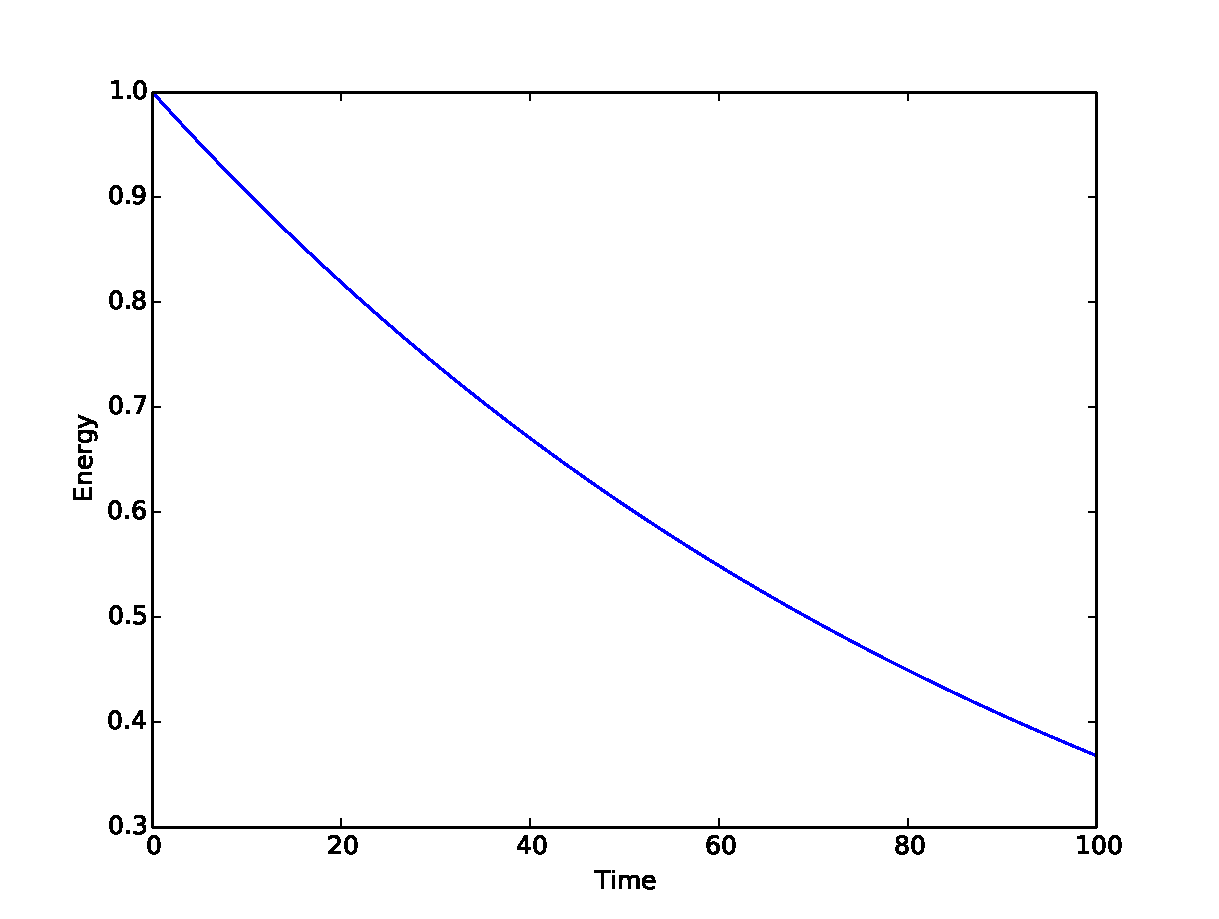
\includegraphics[width=2in]{energy_i.pdf}
		\caption{Energy vs Time}
		\label{fig:energy_i}
		\end{subfigure}
		~
		\begin{subfigure}{0.4\linewidth}
		\centering
		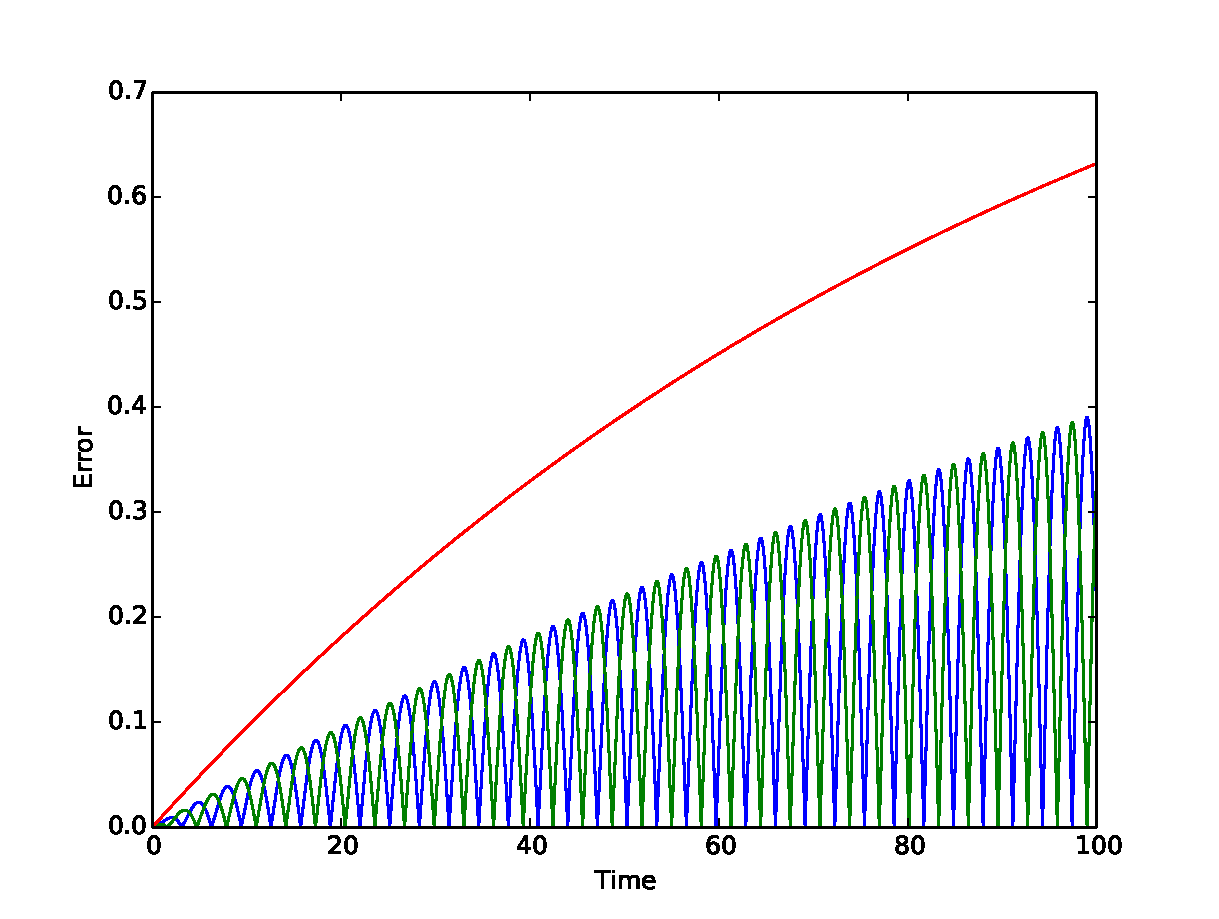
\includegraphics[width=2in]{energyerror_i.pdf}
		\caption{Errors vs Time}
		\label{fig:errors_i}
		\end{subfigure}
		
		\caption{Implicit Energy and Errors vs Time}
	\end{figure}
	
\end{enumerate}



\end{document}